\begin{example}[Viscous Burgers 2D]
\label{ex:kucera}
Based on example in \cite[Section 1.6]{Kucera},
we will solve equation \eqref{eq:ex_burgers} in $\Omega = \langle 0, 1 \rangle^2$.
%\begin{equation}
%		\pdiff{u}{t} + \frac{1}{2}\left(\pdiff{u^2}{x} + \pdiff{u^2}{y}\right)  - 
%		D \cdot \left( \pdiff{^2 u}{x^2} + \pdiff{^2 u}{y^2} \right) 
%		= g
%\end{equation}
%where $D$ is diffusion coefficient and $g$ is a source function. 
We setup boundary condition and source function in such way that the exact 
solution $u_{exact}$ is
\begin{equation}
	u_{exact} =  \ -{\left(e^{\left(-t\right)} - 1\right)} {\left(\sin\left(5 \,x 
	y\right) + \sin\left(-4 \, 
	x y + 4 \,x + 4 \, y\right)\right)}
\end{equation}
We omit analytical forms of $g$ and boundary conditions for brevity.
Different values of coefficient $C_w$ in penalty term then yield only slightly different 
convergence behavior as demonstrated in Figure \ref{fig:kucera_conv} and 
\Cref{fig:kucera_orders}. In this case the solution does not feature any sharp steps and 
increase in penalty coefficient leads to increase in accuracy. 
\end{example}

\begin{figure}[h!]
	\centering
	\begin{tabular}{p{0.5\textwidth} p{0.5\textwidth}}
		\vspace{0pt} 
		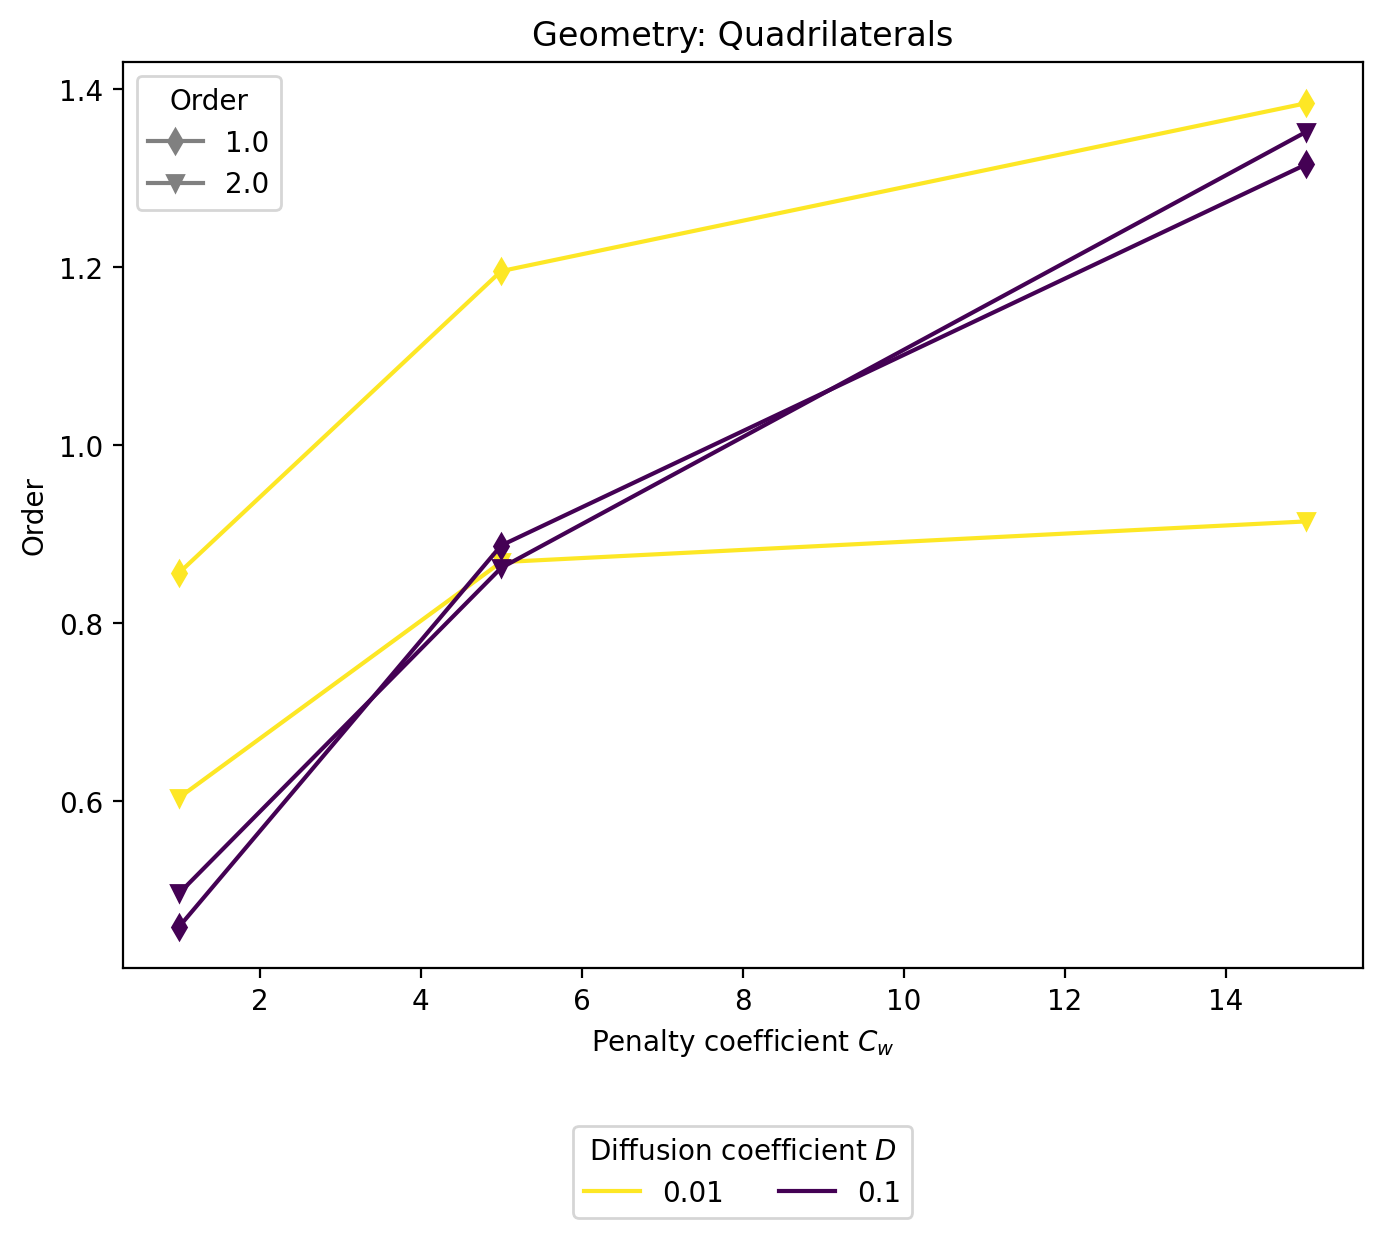
\includegraphics[width=0.49\textwidth]{../figs/parametric/burgers_2D/orders_2_4}
		&
		\vspace{0pt} 
		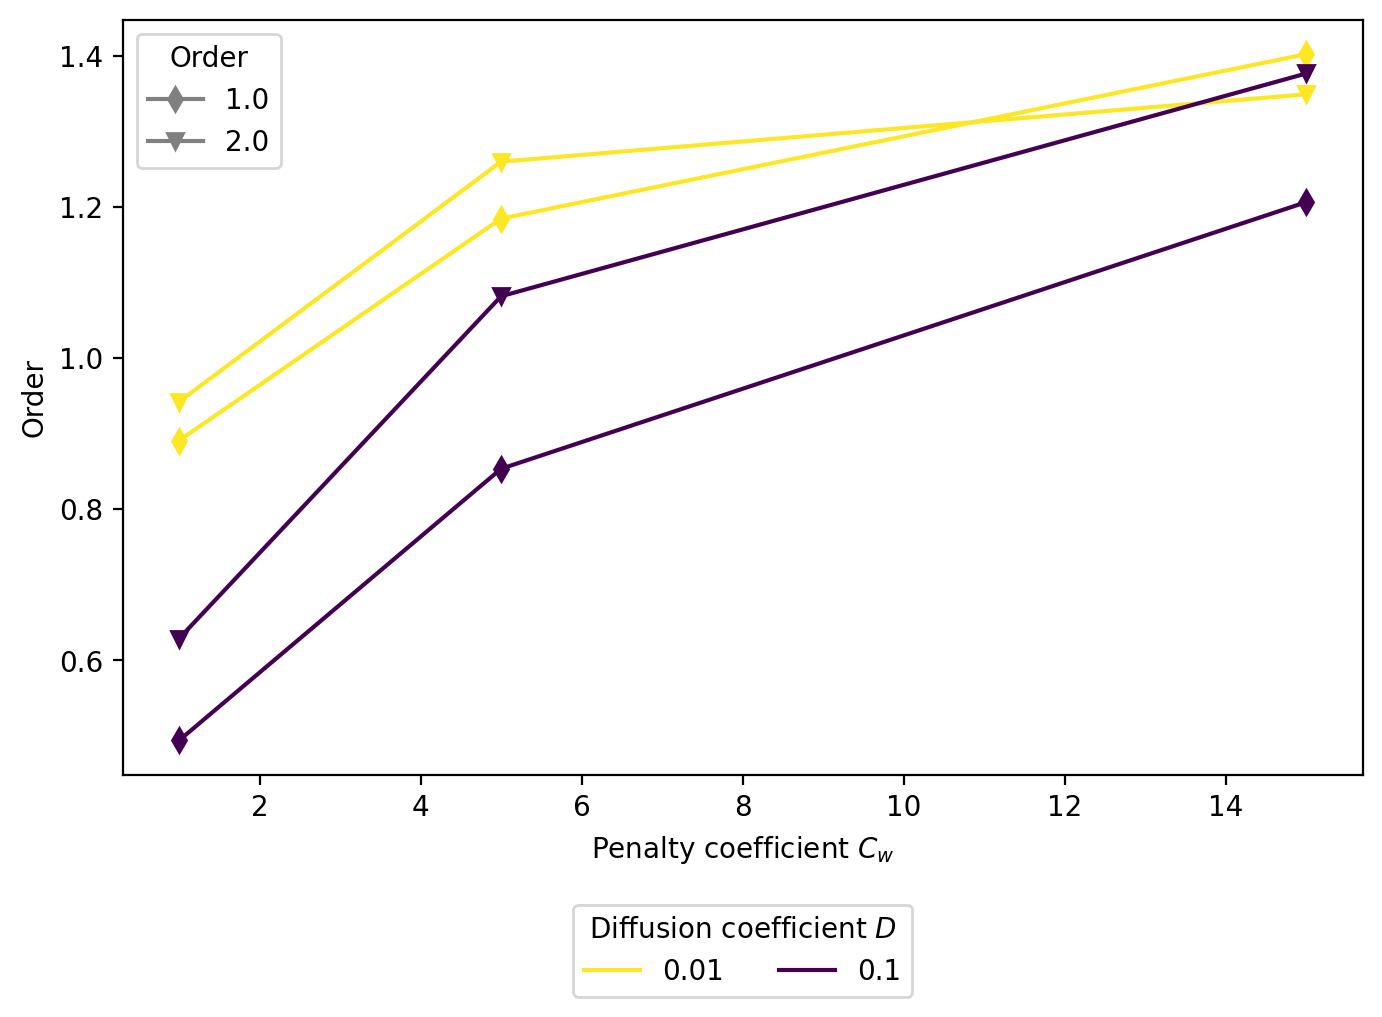
\includegraphics[width=0.49\textwidth]{../figs/parametric/burgers_2D/orders_2_3}
	\end{tabular}
	\caption{\Cref{ex:kucera} average orders for different choice of $C_w$ in 
	tensor-product geometry (left) and simplex geometry (right)}
	\label{fig:kucera_orders}
\end{figure}


\begin{figure}[h!]
	\centering
	\begin{subfigure}{.5\textwidth}	
		\centering	
		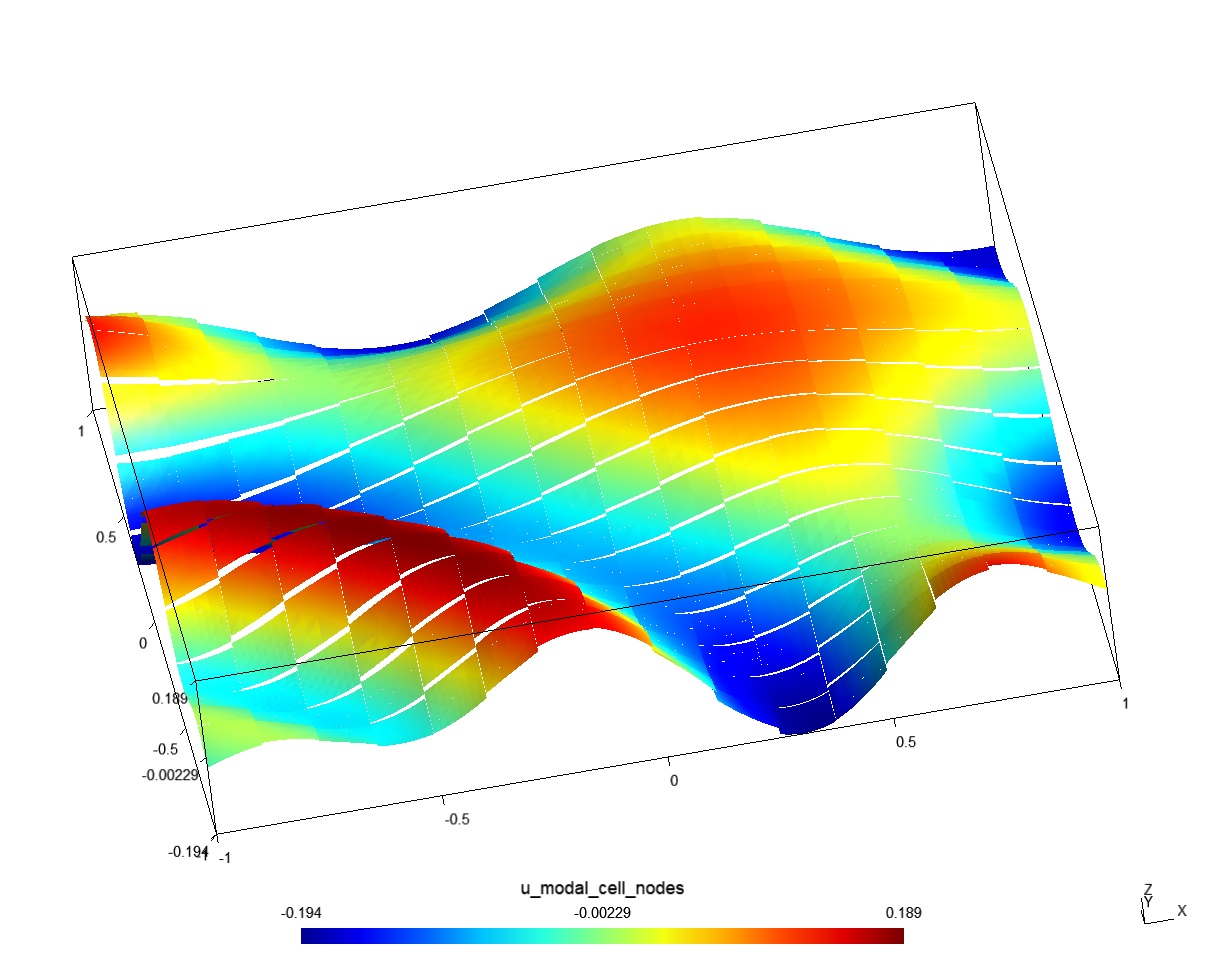
\includegraphics[width=\linewidth]{../figs/err-sols/0_1_0_0_0_0_0_0_0_sol-h256o02.0.png}
		\caption{$C_w = 1$}
	\end{subfigure}%
	\begin{subfigure}{.5\textwidth}
		\centering	
		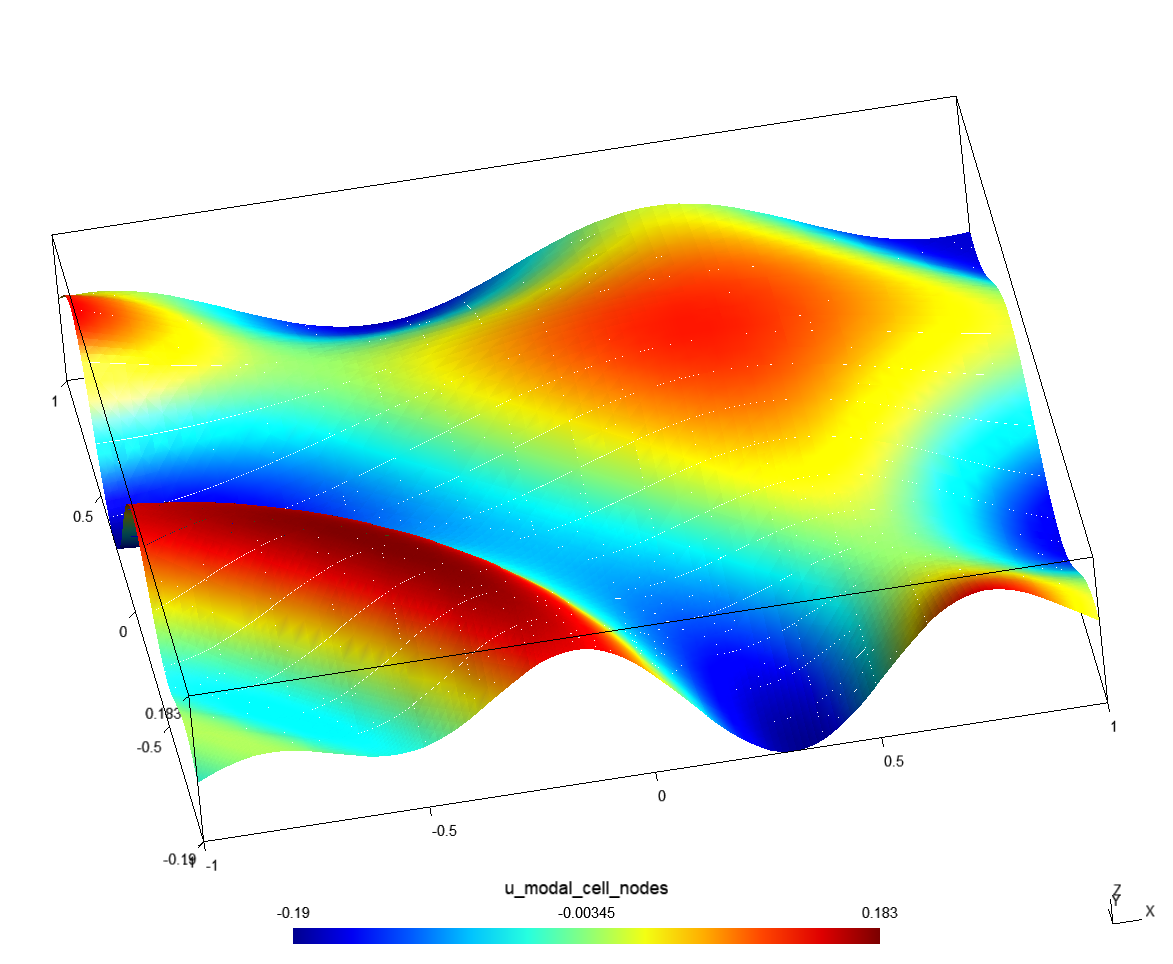
\includegraphics[width=\linewidth]{../figs/err-sols/2_1_2_0_0_0_0_0_0_sol-h256o02.0.png}
		\caption{$C_w = 15$}
	\end{subfigure}
	\caption{Solutions of \Cref{ex:kucera} for different values of $C_w$}
\end{figure}

\begin{figure}[p!]
	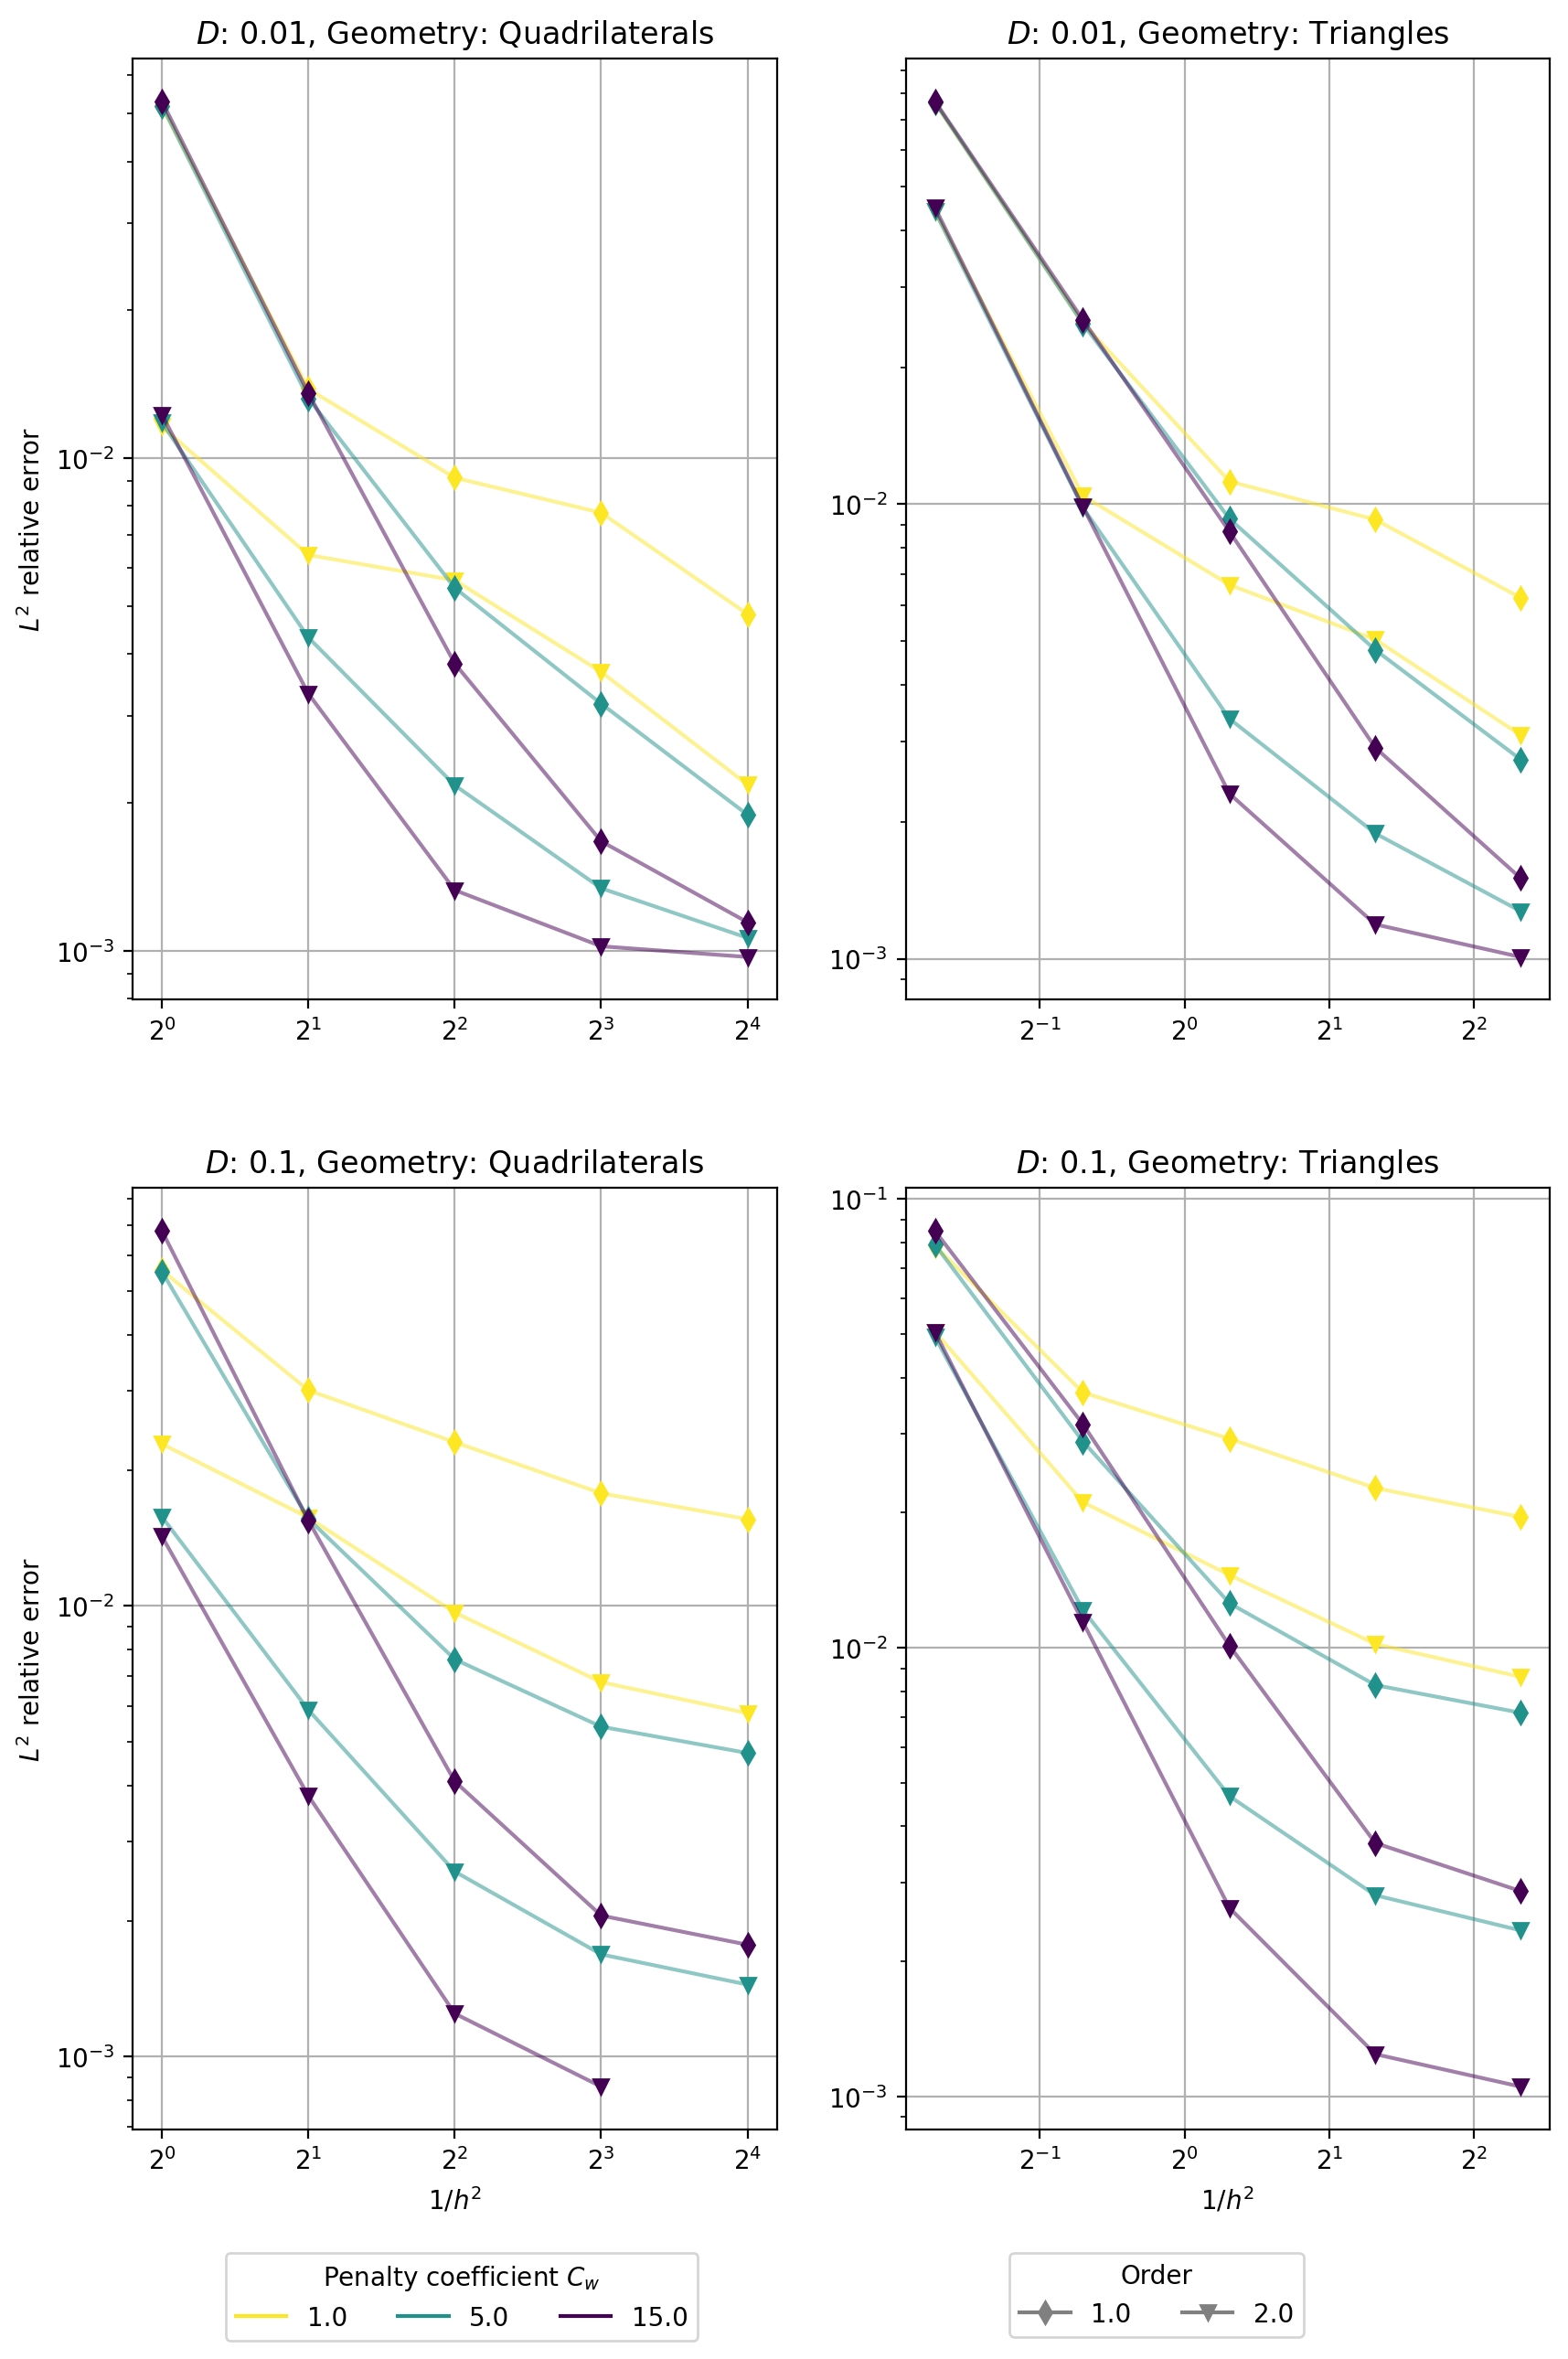
\includegraphics[width=\textwidth]{../figs/parametric/burgers_2D/convergence_symmetry}
	\caption{\Cref{ex:kucera} convergence plots for different choice of $C_w$}
	\label{fig:kucera_conv}
\end{figure}